% tempalte.tex
% Author: 傅申
% 本文件是 实验报告模板.docx 与 实验报告模板.tex 的衍生作品,其著作权属于中国科学技术大学计算机实验教学中心.

% 本文件可使用TeXLive发行版(作者使用的是TeXLive 2021,但理论上2016及以后均可)的xelatex命令编译.
\documentclass[UTF8,fontset=fandol]{ctexart}
\usepackage{LabReport}
\usepackage{amsmath}

\begin{document}
\maketitle{简单组合逻辑电路}


\section*{实验目的}
%列举本实验的实验目的,除指导书上列出的之外,鼓励自行总结及扩展。
\begin{itemize}
  \item 熟练掌握 Logisim 的基本用法
  \item 进一步熟悉 Logisim 更多功能
  \item 用 Logisim 设计组合逻辑电路并进行仿真
  \item 初步学习 Verilog 语法
\end{itemize}


\section*{实验环境}
%列举本实验所用到的各种软硬件环境,如EDA工具、实验平台、实验设备等。
\begin{itemize}
  \item Windows PC 一台: CPU 为 Intel i5-1035G1
  \item Logisim 仿真工具
  \item Xilinx Vitis and Vivado ML Edition 2021.1 与 Micorsoft Visual Studio Code
\end{itemize}


\section*{实验过程}
%按照实验手册的指导,将【实验步骤】部分自己完成一遍,并将过程以图文并茂的形式体现在本报告中。
\begin{ExSteps}
  \step 用真值表自动生成电路\\
  在 Logisim 中新建电路 Step.1. , 然后在画布上放置 4 个输入引脚和 4 个输出引脚, 分别标上标号 I1 - I4, O1 - O4, 并按高低位顺序排列.
  点击菜单栏的 ``Project'' $\rightarrow$ ``Analyze Circuit'' 选项, 在弹出的窗口中选择 ``Table'' 选项, 点击相应的位置修改输出值 (如图\ref{Fig.1.1}),
  点击 ``Build Circuit'' 即可生成电路, 如图\ref{Fig.1.2}.
  
  \begin{figure}[H]
    \centering
    \label{Fig.1}
    \subfigure[真值表]{
      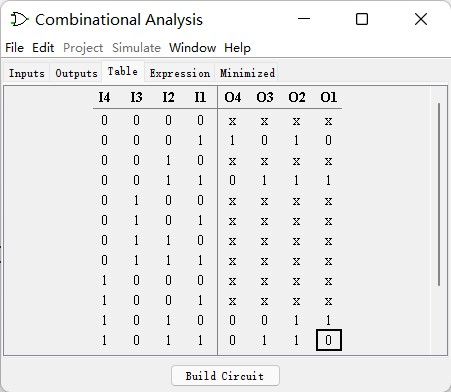
\includegraphics[width = .3\linewidth]{images/Fig.1.1.jpg}
      \label{Fig.1.1}
    }
    \subfigure[电路]{
      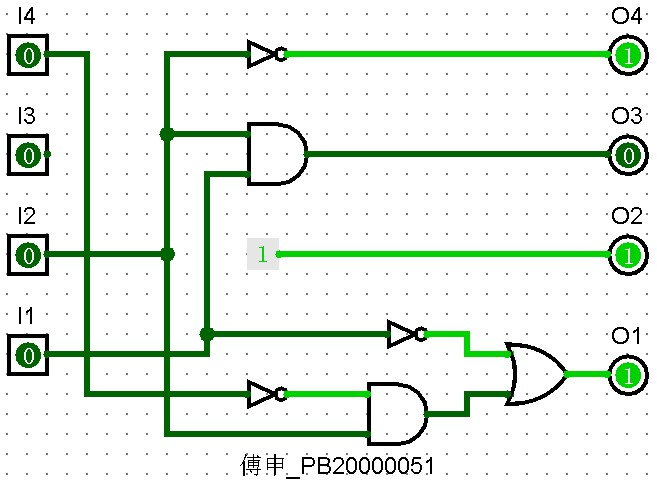
\includegraphics[width = .35\linewidth]{images/Fig.1.2.jpg}
      \label{Fig.1.2}
    }
    \caption{用真值表自动生成电路}
  \end{figure}

  \step 用表达式生成电路图\\
  当输入信号比较多时, 编辑真值表也是比较繁重, 这时我们可以通过表达式生成电路. 比如要生成一个 8 位的优先编码选择器, 其真值表有 256 项之多, 但我们可以很快的写出其表达式:
  \begin{align*}
      y_2 &= i_7 + \overline{i_7}\cdot i_6 + \overline{i_7}\cdot \overline{i_6}i_5 + \overline{i_7}\cdot \overline{i_6}\cdot \overline{i_5}i_4 \\
      y_1 &= i_7 + \overline{i_7}\cdot i_6 + \overline{i_7}\cdot \overline{i_6}\cdot \overline{i_5}\cdot \overline{i_4}\cdot i_3 + \overline{i_7}\cdot \overline{i_6}\cdot \overline{i_5}\cdot \overline{i_4}\cdot \overline{i_3}\cdot i_2 \\
      y_0 &= i_7 + \overline{i_7}\cdot i_6 + \overline{i_7}\cdot \overline{i_6}\cdot \overline{i_5}\cdot \overline{i_4}\cdot i_3 + \overline{i_7}\cdot \overline{i_6}\cdot \overline{i_5}\cdot \overline{i_4}\cdot \overline{i_3}\cdot \overline{i_2}\cdot i_1 
  \end{align*}

  在 Logisim 的画布上放置相应的输入和输出引脚, 然后点击菜单栏的 ``Project'' $\rightarrow$ ``Analyze Circuit'' 选项, 在弹出的窗口中选择 ``Expression'' 选项, 填入每个输出信号的表达式如下:
  
  \begin{lstlisting}[basicstyle = \small\ttfamily]
  y2 = i7 + ~i7 i6 + ~i7 ~i6 i5 + ~i7 ~i6 ~i5 i4
  y1 = i7 + ~i7 i6 + ~i7 ~i6 ~i5 ~i4 i3 + ~i7 ~i6 ~i5 ~i4 ~i3 i2
  y0 = i7 + ~i7 ~i6 i5 + ~i7 ~i6 ~i5 ~i4 i3 + ~i7 ~i6 ~i5 ~i4 ~i3 ~i2 i1    
  \end{lstlisting}
  
  最后点击 ``Build Circuit'' 生成电路, ``Expression'' 选项卡和生成的电路如下图\ref{Fig.2}.

  \begin{figure}[H]
    \centering
    \subfigure[``Expression'' 选项卡]{
      \label{Fig.2.1}
      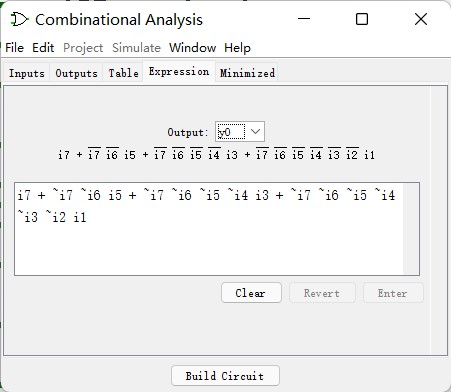
\includegraphics[width = .3\linewidth]{images/Fig.2.1.jpg}
    }
    \subfigure[生成的电路]{
      \label{Fig.2.2}
      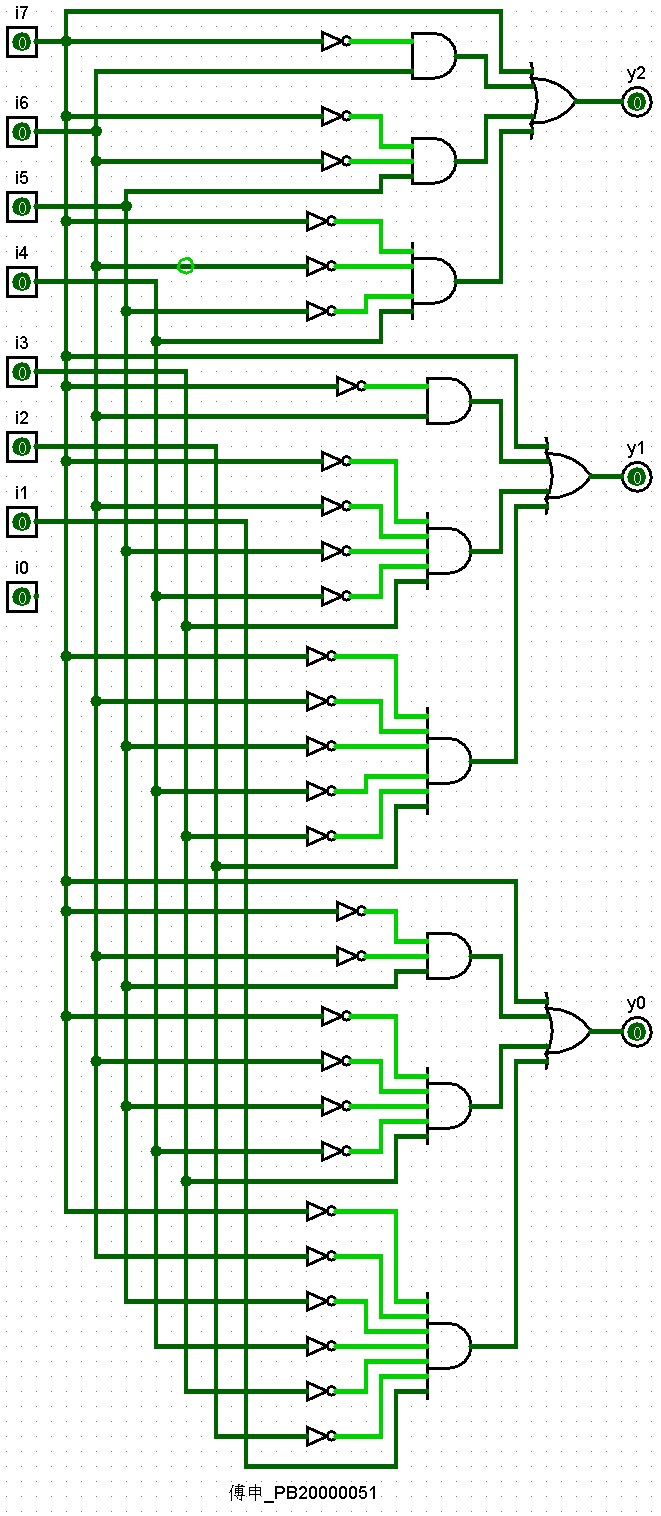
\includegraphics[width = .2\linewidth]{images/Fig.2.2.jpg}
    }
    \caption{用表达式生成电路图}
    \label{Fig.2}
  \end{figure}

  可以看出该电路占用的逻辑门较多, 这时可以借助窗口中的 ``Minimized'' 的选项卡来对表达式和电路进行简化, 如图\ref{Fig.3} 中的
  化简后的与或式和或与式结构.

  \begin{figure}[H]
    \centering
    \subfigure[与或式]{
      \label{Fig.3.1}
      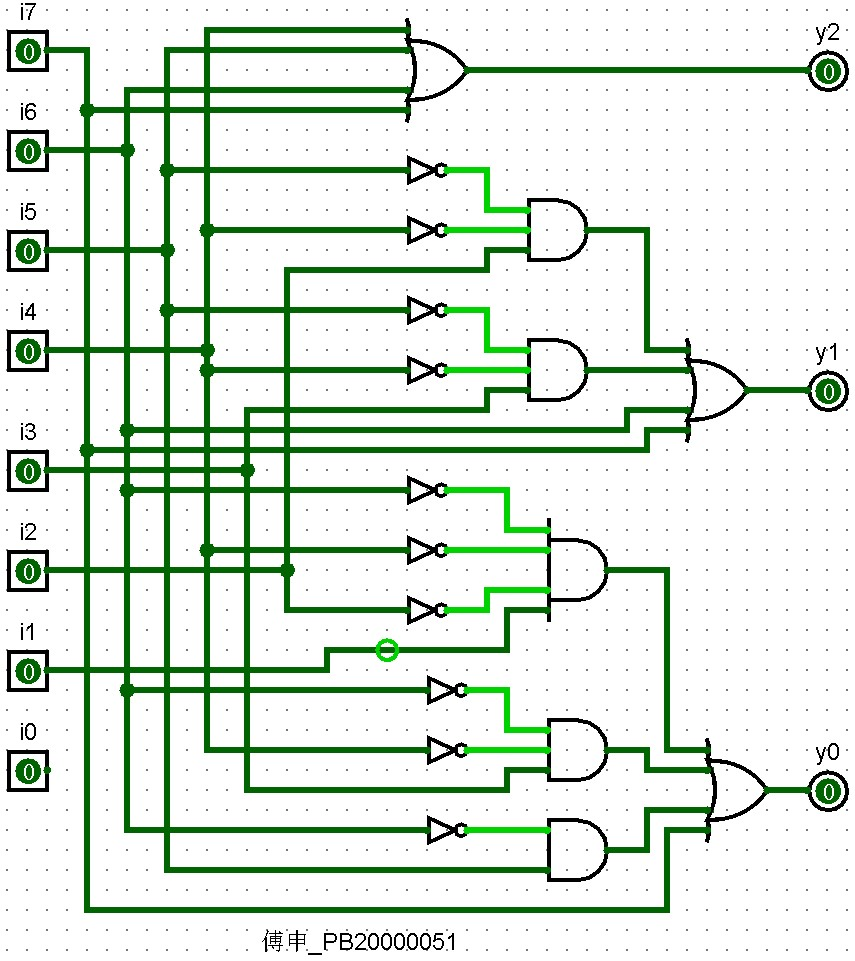
\includegraphics[width = .3\linewidth]{images/Fig.3.1.jpg}
    }
    \subfigure[或与式]{
      \label{Fig.3.2}
      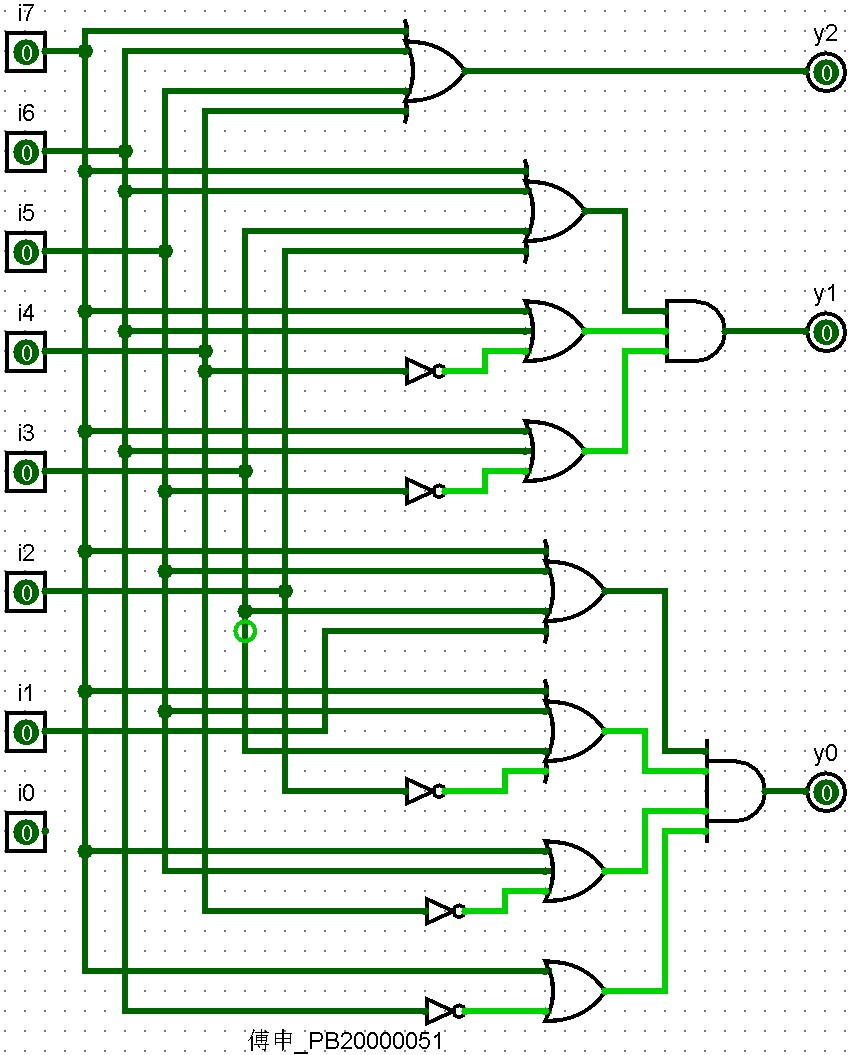
\includegraphics[width = .27\linewidth]{images/Fig.3.2.jpg}
    }
    \caption{简化后的电路}
    \label{Fig.3}
  \end{figure}
\newpage
  \step Verilog HDL 语法入门 \\
  Verilog 模块的最基本结构如下代码 \ref{Code.1}.
  \begin{lstlisting}[style=verilogstyle, caption={Verilog模块基本结构}, label={Code.1}]
module 模块名(
  输入端口声明,
  输出端口声明
);
  内部信号声明<可选>;

  逻辑描述(模块主体)
endmodule

// 单行注释
/*
   多行注释
 */
  \end{lstlisting}
比如我们要实现一个半加器, 其 Verilog 代码就如下代码 \ref{Code.2}, 其中 \texttt{add} 模块从行为级上进行描述, 而 \texttt{add1} 模块则从门电路层次进行描述.
\begin{lstlisting}[style=verilogstyle, caption={半加器模块}, label={Code.2}]
  // 从行为级上描述
module add(
    input a, b,
    output sum, cout
    );
    assign {cout,sum} = a + b; // 位拼接
endmodule

// 从电路级上描述
module add1(
    input a,b,
    output sum,cout
    );
    // 两个 assign 是位置无关的
    assign cout = a & b;
    assign sum  = a ^ b;
endmodule
    \end{lstlisting}
    而要使用已经设计了的模块, 我们可以在代码中调用该模块. 比如我们要使用半加器来构造一个全加器, 其 Verilog 代码就如代码\ref{Code.3}.
    \newpage
    \begin{lstlisting}[style=verilogstyle, caption={全加器}, label={Code.3}]
module full_add(
    input a,b,cin,
    output sum,cout
    );
    wire s,carry1,carry2; // 内部信号声明
    // 调用半加器
    add add_inst1( 
        .a (a ),
        .b (b ),
        .sum (s ),
        .cout (carry1)
        );
    add add_inst2(
        .a (s ),
        .b (cin ),
        .sum (sum ),
        .cout (carry2)
        );
    assign cout = carry1 | carry2;
endmodule
    \end{lstlisting}
  \end{ExSteps}


\section*{实验练习}
%如无特殊说明,则应完成对应实验手册上的所有练习题目,将过程和结果以图文并茂的形式体现在本报告中,建议实验过程中随手保存各种截图。
\begin{ExQuestions}
  \question 在 Logisim 中新建电路, 在画布上放置 3 个输入引脚和 2 个输出引脚, 并标上标号, 打开 ``table'' 选项卡, 编辑真值表如下图 \ref{Fig.4.1}, 点击 ``Build Circuit'', 生成的电路如下图 \ref{Fig.4.2}.
  \begin{figure}[H]
    \centering
    \label{Fig.4}
    \subfigure[真值表]{
      \label{Fig.4.1}
      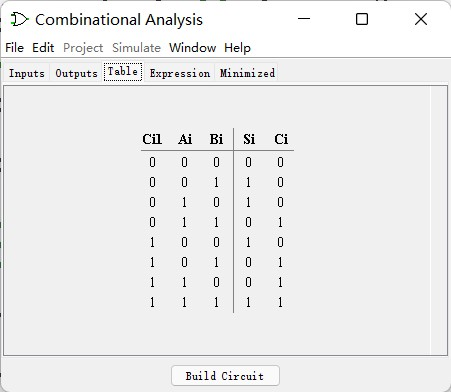
\includegraphics[width = .4\linewidth]{images/Fig.4.1.jpg}
    }
    \subfigure[电路]{
      \label{Fig.4.2}
      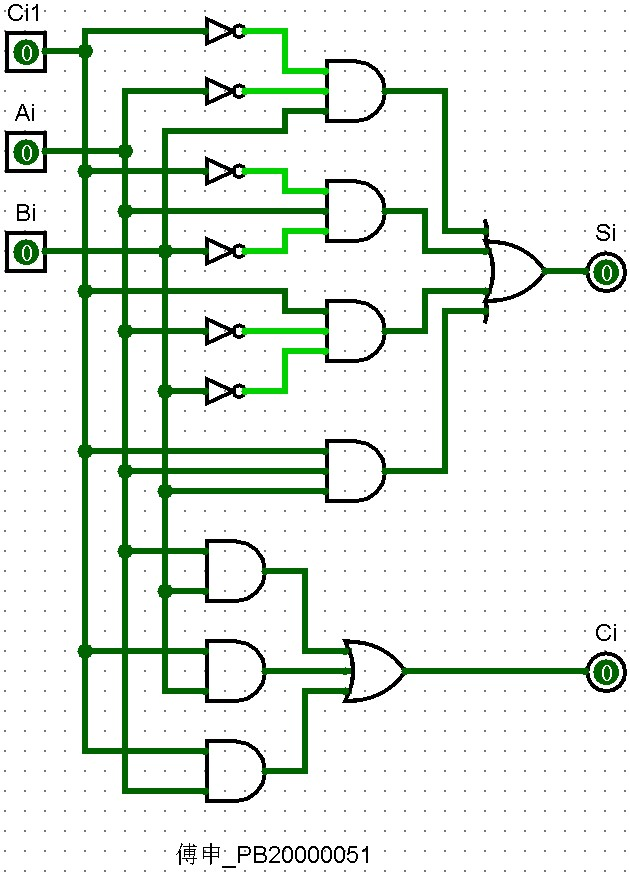
\includegraphics[width = .3\linewidth]{images/Fig.4.2.jpg}
    }
    \caption{题目 1 中的真值表和电路}
  \end{figure}
  \newpage
  \question 分析下面的真值表, 列出下面的逻辑表达式:
  \begin{align*}
    Y_7 &= \overline{G_1} + {G_2} + {G_3} + \overline{A_2} + \overline{A_1} + \overline{A_0} \\
    Y_6 &= \overline{G_1} + {G_2} + {G_3} + \overline{A_2} + \overline{A_1} + {A_0} \\
    Y_5 &= \overline{G_1} + {G_2} + {G_3} + \overline{A_2} + {A_1} + \overline{A_0} \\
    Y_4 &= \overline{G_1} + {G_2} + {G_3} + \overline{A_2} + {A_1} + {A_0} \\
    Y_3 &= \overline{G_1} + {G_2} + {G_3} + {A_2} + \overline{A_1} + \overline{A_0} \\
    Y_2 &= \overline{G_1} + {G_2} + {G_3} + {A_2} + \overline{A_1} + {A_0} \\
    Y_1 &= \overline{G_1} + {G_2} + {G_3} + {A_2} + {A_1} + \overline{A_0} \\
    Y_0 &= \overline{G_1} + {G_2} + {G_3} + {A_2} + {A_1} + {A_0}
  \end{align*}
  在 Logisim 中新建电路, 在画布上放置 6 个输入引脚和 8 个输出引脚, 并标上标号, 打开 ``Expression'' 标签卡, 填入每个输出信号的表达式如下:
  \begin{lstlisting}[basicstyle = \small\ttfamily]
Y7 = ~G1 + G2 + G3 + ~A2 + ~A1 + ~A0
Y6 = ~G1 + G2 + G3 + ~A2 + ~A1 + A0
Y5 = ~G1 + G2 + G3 + ~A2 + A1 + ~A0
Y4 = ~G1 + G2 + G3 + ~A2 + A1 + A0
Y3 = ~G1 + G2 + G3 + A2 + ~A1 + ~A0
Y2 = ~G1 + G2 + G3 + A2 + ~A1 + A0
Y1 = ~G1 + G2 + G3 + A2 + A1 + ~A0
Y0 = ~G1 + G2 + G3 + A2 + A1 + A0
  \end{lstlisting}
  点击 ``Build Circuit'' 按钮,生成的电路如图 \ref{Fig.5.1}, 转到 ``Table'' 选项卡, Logisim 分析出的部分电路真值表如图 \ref{Fig.5.2}.
  \begin{figure}[H]
    \centering
    \label{Fig.5}
    \subfigure[生成的电路]{
      \label{Fig.5.1}
      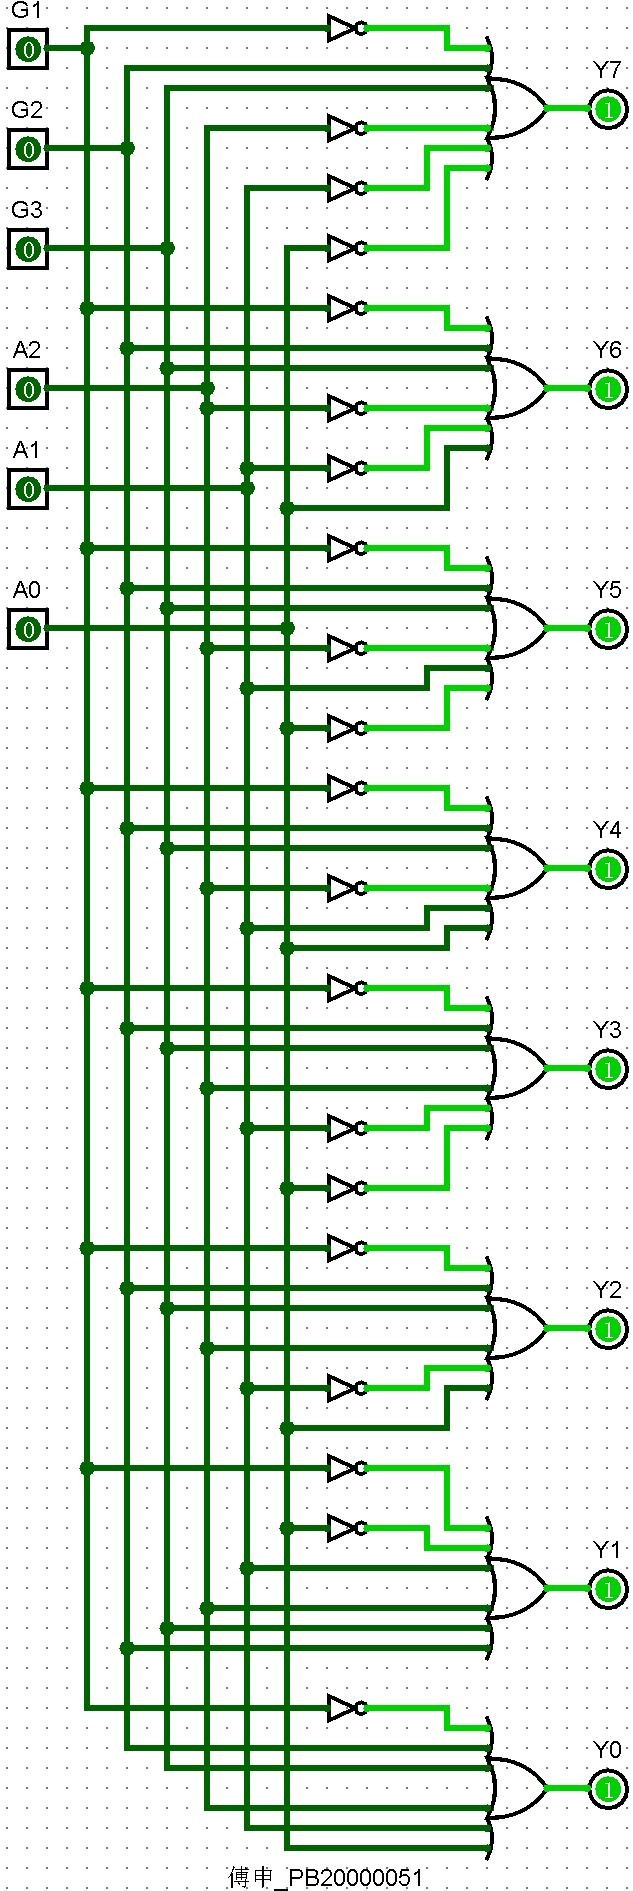
\includegraphics[width = .225\linewidth]{images/Fig.5.1.jpg}
    }
    \subfigure[部分真值表]{
      \label{Fig.5.2}
      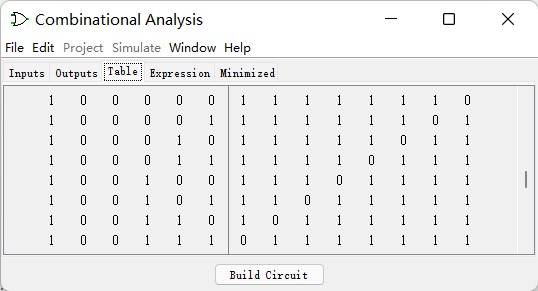
\includegraphics[width = .6\linewidth]{images/Fig.5.2.jpg}
    }
    \caption{题目 2 中的电路}
  \end{figure}
  \newpage
  \question 使用 Logisim 绘制 1 bit 位宽的二选一选择器电路图如图 \ref{Fig.6}, 根据该电路图, 编写的 Verilog 代码如下代码 \ref{Code.4}.
  \begin{figure}[H]
    \centering
    \label{Fig.6}
    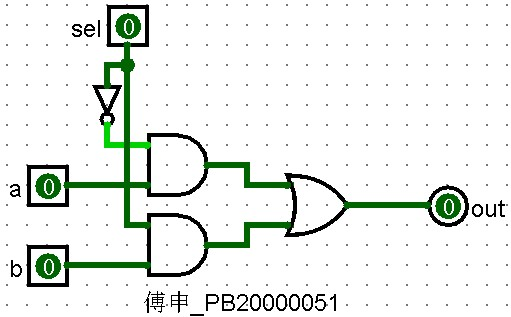
\includegraphics[width = .5\linewidth]{images/Fig.6.jpg}
    \caption{1 bit 位宽的二选一选择器电路}
  \end{figure}
  \begin{lstlisting}[style=verilogstyle, caption={1 bit 位宽的二选一选择器}, label={Code.4}]
module MUX_1bit_2to1 (
    input i0, i1, sel,
    output out
);
    assign out = (~sel & i0) | (sel & i1);
endmodule
  \end{lstlisting}

  \question 通过例化题目 3 中的二选一选择器, 在四选一选择器中调用该模块, 先对高位进行选择, 在对低位进行选择, 如代码 \ref{Code.5}.
  \begin{lstlisting}[style=verilogstyle, caption={1 bit 位宽的四选一选择器}, label={Code.5}]
module MUX_1bit_4to1 (
    input a, b, c, d, sel1, sel0,
    output out
);
    wire low_bit_0, low_bit_1;

    MUX_1bit_2to1 Mux0(
        .i0 (a),
        .i1 (c),
        .sel(sel1),
        .out(low_bit_0)
    );
    MUX_1bit_2to1 Mux1(
        .i0 (b),
        .i1 (d),
        .sel(sel1),
        .out(low_bit_1)
    );
    
    MUX_1bit_2to1 Mux2(
        .i0 (low_bit_0),
        .i1 (low_bit_1),
        .sel(sel0),
        .out(out)
    );
endmodule
  \end{lstlisting}
对应的电路图如图\ref{Fig.7}.
  \begin{figure}[H]
    \centering
    \label{Fig.7}
    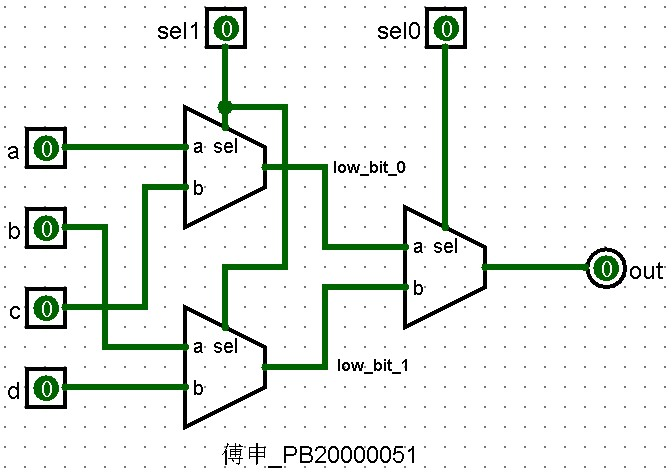
\includegraphics[width = .5\linewidth]{images/Fig.7.jpg}
    \caption{1 bit 位宽的四选一选择器电路}
  \end{figure}
  \question 使用化简后的逻辑表达式:
  \begin{align*}
    y_2 &= i_7 + i_6 + i_5 + i_4\\
    y_1 &= i_7 + i_6 + \overline{i_5} \cdot \overline{i_4} \cdot i_3 + \overline{i_5} \cdot \overline{i_4} \cdot i_2\\
    y_0 &= i_7 + \overline{i_6} \cdot i_5 + \overline{i_6} \cdot \overline{i_4} \cdot i_3 + \overline{i_6} \cdot \overline{i_4} \cdot \overline{i_2} \cdot i_1
  \end{align*}
  可以编写出八位优先编码器的 Verilog 代码如下代码 \ref{Code.6}.
  \begin{lstlisting}[style=verilogstyle, caption={八位优先编码器}, label={Code.6}]
module priority_encoder_8bit (
    input i7, i6, i5, i4, i3, i2, i1, i0,
    output y2, y1, y0
);
    assign y2 = i7 | i6 | i5 | i4;
    assign y1 = i7 | i6 | (~i5 & ~i4 & i3) | (~i5 & ~i4 & i2);
    assign y0 = i7 | (~i6 & i5) | (~i6 & ~i4 & i3) | 
                (~i6 & ~i4 & ~i2 & i1);
endmodule
  \end{lstlisting}
  \question 分析 Verilog 代码, 可以知道 $s_1, s_2$ 的表达式为:
  \begin{align*}
    s_1 &= \overline{a} \cdot \overline{b} \cdot c + \overline{a} \cdot b \cdot \overline{c} + a \cdot \overline{b} \cdot \overline{c} + a\cdot b \cdot c = (a\oplus b)\oplus c\\
    s_2 &= \overline{a} \cdot b \cdot c + a \cdot \overline{b} \cdot c + a \cdot b \cdot \overline{c} + \overline{a} \cdot \overline{b} \cdot \overline{c} = \overline{(a\oplus b)\oplus c}
  \end{align*}
  得出真值表如下表\ref{Tab.1}.
  \begin{table}[!ht]
    \centering
    \label{Tab.1}
    \caption{Verilog 代码真值表}
    \begin{tabular}{ccc|cc} 
    \toprule
    $a$ & $b$ & $c$ & $s_1$ & $s_2$  \\ 
    \hline
    0   & 0   & 0   & 0     & 1      \\
    0   & 0   & 1   & 1     & 0      \\
    0   & 1   & 0   & 1     & 0      \\
    0   & 1   & 1   & 0     & 1      \\
    1   & 0   & 0   & 1     & 0      \\
    1   & 0   & 1   & 0     & 1      \\
    1   & 1   & 0   & 0     & 1      \\
    1   & 1   & 1   & 1     & 0      \\
    \bottomrule
    \end{tabular}
    \end{table}
    可以看出, 当 $a, b, c$ 中有奇数个 1 时, $s_1$ 为 1, $s_2$ 为 0; 当 $a, b, c$ 中有偶数个 1 时 (或全为 0 时), $s_1$ 为 0, $s_2$ 为 1. 因此, 该 Verilog 代码的功能是统计 $a, b, c$ 中 1 的个数是奇数还是偶数. 对应的电路图如图 \ref{Fig.8}.
    \begin{figure}[H]
      \centering
      \label{Fig.8}
      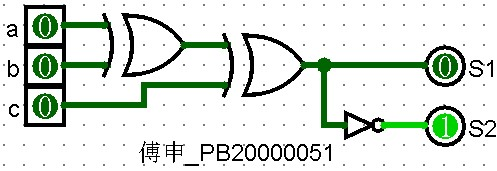
\includegraphics[width = .5\linewidth]{images/Fig.8.jpg}
      \caption{Verilog 代码对应的电路图}
    \end{figure}
\end{ExQuestions}
\section*{总结与思考}
%请填写对于本次实验的总结与思考,鼓励填写对于本实验或者本课程的各种建议和吐槽。
\begin{description}
  \item[收获] 了解了在 Logisim 中如何通过真值表和表达式生成组合逻辑电路以及如何简化电路, 入门了 Verilog HDL 语言.
  \item[难易程度与任务量] 较轻松.
  \item[建议] 暂无. 
\end{description}
\end{document}
